\documentclass[
      12pt,
        ]{article}






% --- type and typeface? -----------------------

% input
\usepackage[utf8]{inputenc}

% typography
\usepackage{microtype}


\usepackage[T1]{fontenc}


% text block
\usepackage{setspace}
\usepackage[              left = 1in,top = 1in,right = 1in,bottom = 1in             ]{geometry}

\usepackage{enumitem}
  \setlist{noitemsep}



% decimal numbering for appendix figs and tabs


% Deletes section counters
% \setcounter{secnumdepth}{0}







  \usepackage{longtable, booktabs}

  \usepackage{graphicx,grffile}
  % Scale images; don't overflow page margins by default.
  % Still possible explicate \includegraphics[width, height, ...]{}
  \makeatletter
    \def\maxwidth{\ifdim\Gin@nat@width>\linewidth\linewidth\else\Gin@nat@width\fi}
    \def\maxheight{\ifdim\Gin@nat@height>\textheight\textheight\else\Gin@nat@height\fi}
  \makeatother 
  \setkeys{Gin}{width=\maxwidth,height=\maxheight,keepaspectratio}










% 

% \newtheorem{hypothesis}{Hypothesis}

\makeatletter
  \@ifpackageloaded{hyperref}{}{%
    \ifxetex
      % page size defined by xetex
      % unicode breaks when used with xetex
      \PassOptionsToPackage{hyphens}{url}\usepackage[setpagesize = false, 
                                                     unicode = false, 
                                                     xetex]{hyperref}
    \else
      \PassOptionsToPackage{hyphens}{url}\usepackage[unicode = true]{hyperref}
    \fi
  }

  \@ifpackageloaded{color}{
    \PassOptionsToPackage{usenames,dvipsnames}{color}
  }{
    \usepackage[usenames,dvipsnames]{color}
  }
\makeatother

\hypersetup{breaklinks = true,
            bookmarks = true,
            pdfauthor = {},
             pdfkeywords  =  {},  
            pdftitle = {Do Private Regulations Ratchet Up?: A comparative classification framework},
            colorlinks = true,
            citecolor = blue,
            urlcolor = blue,
            linkcolor = magenta,
            pdfborder = {0 0 0}}

% \urlstyle{same}  % don't use monospace font for urls


% set default figure placement to htbp
\makeatletter
  \def\fps@figure{hbtp}
\makeatother


% optional footnotes as endnotes


% ----- Pandoc wants this tightlist command ----------
\providecommand{\tightlist}{
  \setlength{\itemsep}{0pt}
  \setlength{\parskip}{0pt}
}





% --- title & section styles -----------------------


% title, author, date
  \title{Do Private Regulations Ratchet Up?: 
           \\ A comparative classification framework}

  \author{}

% auto-format date?
  \date{\today}


% abstract
\usepackage{abstract}
  \renewcommand{\abstractname}{}    % clear the title
  \renewcommand{\absnamepos}{empty} % originally center

  \newcommand*{\authorfont}{\sffamily\selectfont}


% section titles
\usepackage[small, bf, sc]{titlesec}
  % \titleformat*{\subsection}{\itshape}
  \titleformat*{\subsubsection}{\itshape} 
  \titleformat*{\paragraph}{\itshape} 
  \titleformat*{\subparagraph}{\itshape}









\begin{document}
 

% --- PAGE: title and abstract -----------------------

  \maketitle

% \pagenumbering{gobble}




% --- PAGE: contents -----------------------

    \hypersetup{linkcolor = black}
  \setcounter{tocdepth}{2}
  \tableofcontents



% --- PAGE: body -----------------------



\noindent 
    \begin{center}\rule{0.5\linewidth}{\linethickness}\end{center}

\textbf{Abstract}

Scholars present conflicting accounts of change in private regulations,
including whether competing programs ``race to the bottom,'' ``ratchet
up,'' ``converge,'' or ``diverge.'' We find this to be a symptom of
inconsistent measures of regulatory stringency. To remedy this, we offer
a framework to distinguish three often-conflated measures: policy scope,
prescriptiveness, and performance levels. Using our framework, we
compare two leading U.S. forestry certification programs, revealing an
upward but divergent pattern in policy prescriptiveness. The program
founded by activists generally added requirements that impose costs on
firms, while the program established by the American Forest \& Paper
Association generally added requirements that benefit the sector. This
is consistent with our hypothesis that industry-backed programs target
less costly types of regulatory stringency than activist-backed
programs. We also find several more nuanced patterns of change that
previous scholarship failed to anticipate, illustrating how
disentangling types of stringency can improve theory building and
testing,

\begin{center}\rule{0.5\linewidth}{\linethickness}\end{center}

\subsection{Context: Regulating foresty in the
U.S.}\label{context-regulating-foresty-in-the-u.s.}

Competing certification regimes, the Forest Stewardship Council (FSC)
and The Sustainable Forestry Initiative (SFI), play a major role in
regulating the forestry industry in the United States, regulating a
third of commercially harvested timberland including most
corporate-owned timberland.


\includegraphics{images/fsclogo.png}

\includegraphics{images/sfilogo.jpeg}
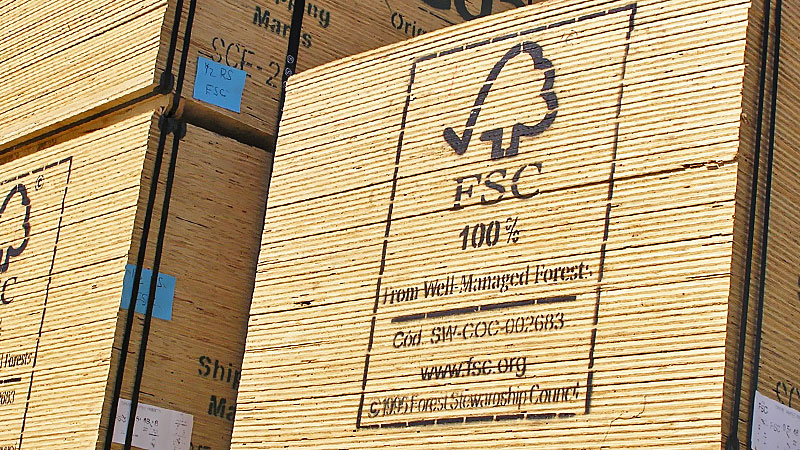
\includegraphics{images/fscwood.jpg}

\subsubsection{U.S. Timberland by ownership and certification
scheme}\label{u.s.-timberland-by-ownership-and-certification-scheme}

\begin{center}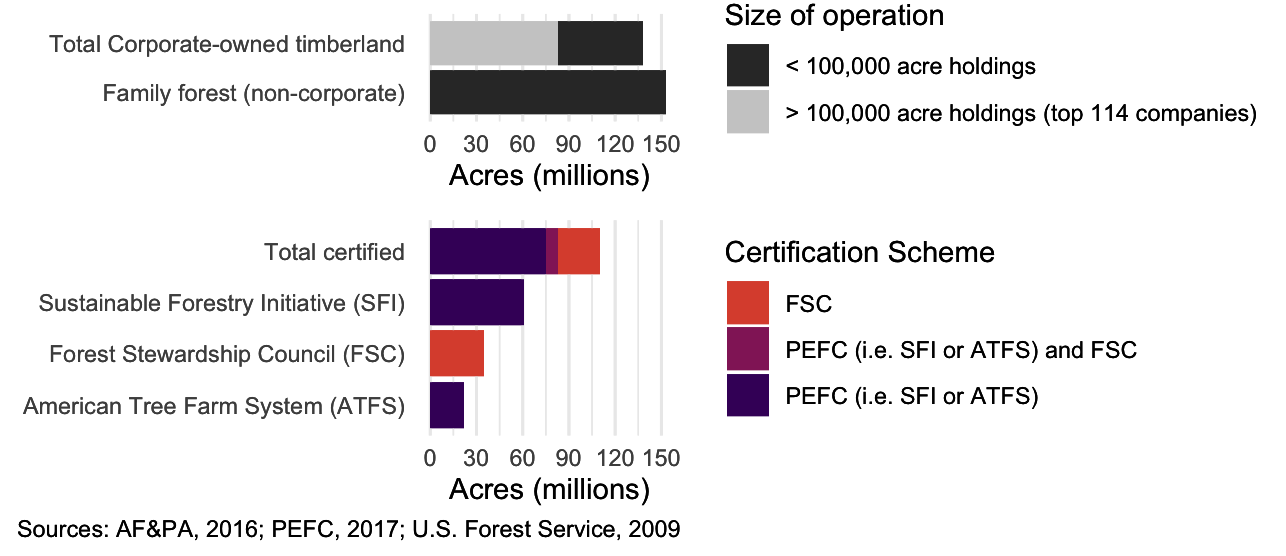
\includegraphics{Figs/acres-1} \end{center}

\begin{center}\rule{0.5\linewidth}{\linethickness}\end{center}

\subsection{Comparing Forest Certification
Programs}\label{comparing-forest-certification-programs}

We each program's stringency on 48 key social and environmental issues.
For example, the FSC and SFI have different limits on the size of
clearcuts and harvesting buffers around streams.

\subsubsection{Limits on clearcut size}\label{limits-on-clearcut-size}

\begin{center}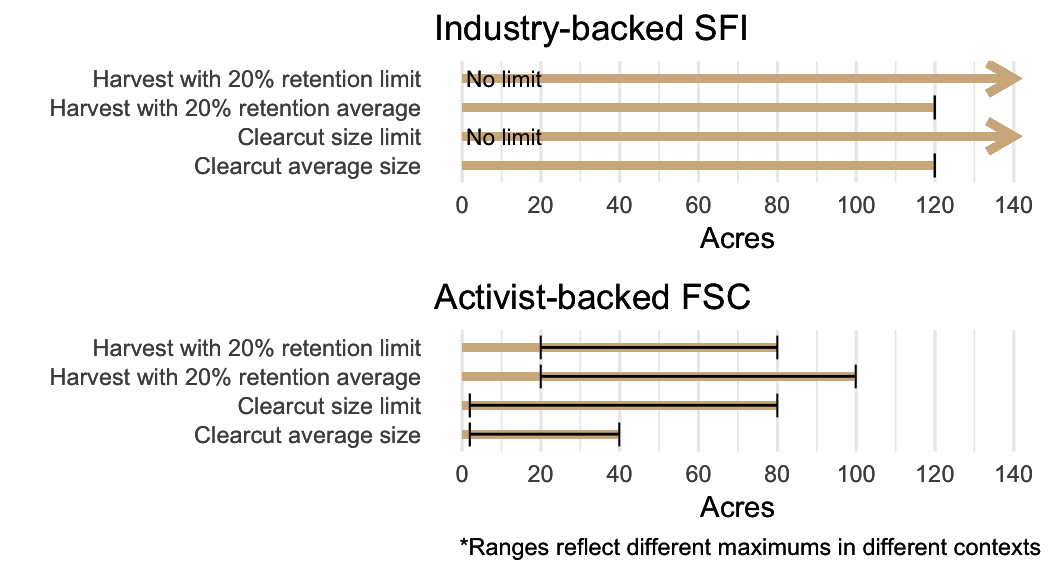
\includegraphics{Figs/clearcuts-1} \end{center}

\subsubsection{Limits on harvesting near
streams}\label{limits-on-harvesting-near-streams}

\begin{center}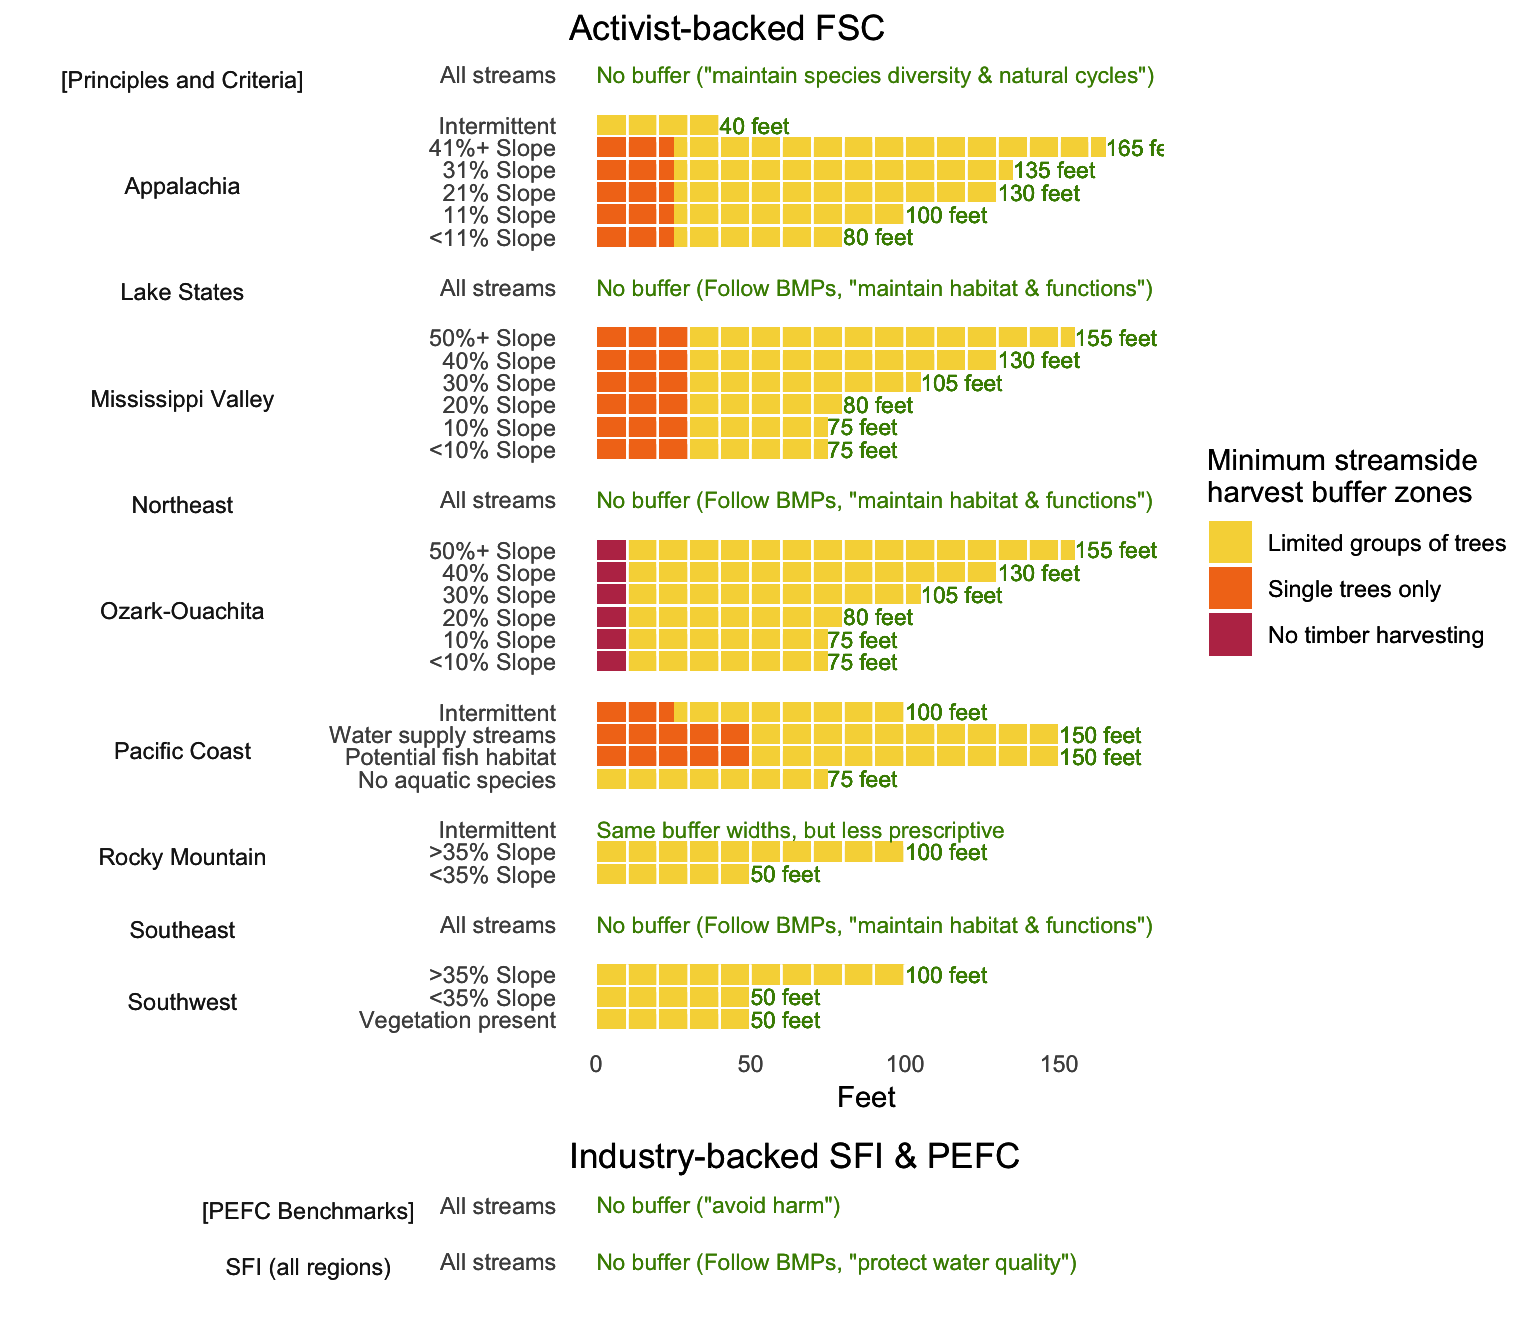
\includegraphics{Figs/riparian-1} \end{center}

\begin{center}\rule{0.5\linewidth}{\linethickness}\end{center}

In addition to issue-by-issue comparisons, we use two measures of
regulatory stringency that can be aggregated across issues: the scope of
issues addressed and the prescriptiveness of requirements on each issue.

\subsubsection{Policy Prescriptiveness}\label{policy-prescriptiveness}

\begin{longtable}[]{@{}lcc@{}}
\toprule
& Discretionary & Non-discretionary\tabularnewline
\midrule
\endhead
Procedural (plan- or systems-based) & Flexible & Somewhat
prescriptive\tabularnewline
Substantive (e.g. a policy threshold) & Flexible & Most
prescriptive\tabularnewline
\bottomrule
\end{longtable}

\begin{center}\rule{0.5\linewidth}{\linethickness}\end{center}

\subsubsection{Scope and Prescriptiveness of FSC-US and SFI
2008-2016}\label{scope-and-prescriptiveness-of-fsc-us-and-sfi-2008-2016}

\begin{center}\includegraphics{Figs/FSC-SFI-1} \end{center}

\begin{center}\rule{0.5\linewidth}{\linethickness}\end{center}

\subsubsection{Scope and Prescriptiveness of FSC P\&C and PEFC
2008-2015}\label{scope-and-prescriptiveness-of-fsc-pc-and-pefc-2008-2015}

\begin{center}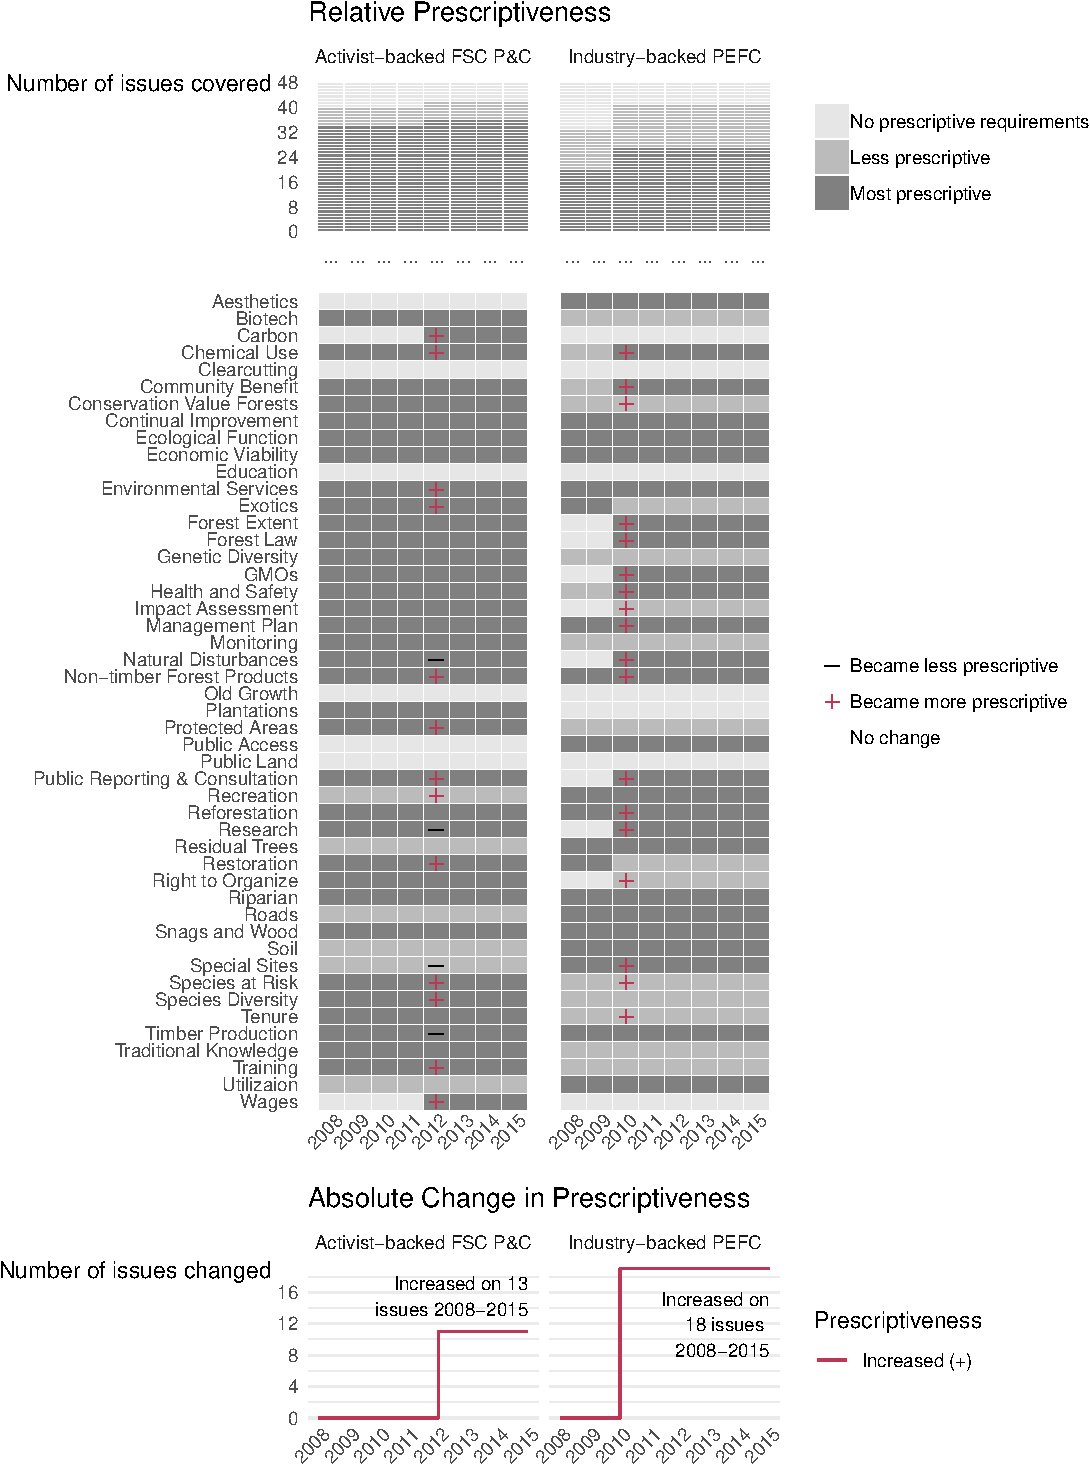
\includegraphics{Figs/FSC-PEFC-1} \end{center}

\begin{center}\rule{0.5\linewidth}{\linethickness}\end{center}

\begin{center}\rule{0.5\linewidth}{\linethickness}\end{center}

\subsubsection{2010 Patterns of change in prescriptiveness among U.S.
Forestry Certification Programs (FSC-US and SFI) on 48 Key
Issues}\label{patterns-of-change-in-prescriptiveness-among-u.s.-forestry-certification-programs-fsc-us-and-sfi-on-48-key-issues}

Upwardly converging issues: Contual Improvement

Upward parallell issues: Public reporting and consultation: Management
plan: Carbon

Upwardly diverging issues: Forest extent: Conservation Value Forests:
Protected areas: Ecosystem function: Clearcutting: Snags and wood:
Plantations: Species at risk: Restoration: NTFP: Soil: Riparian: Public
lands: Genetic diversity: Public access: Residual trees: Utilization:
Education

Opposing diverging issues: Old growth: Aesthetics: Training

Downwardly converging issues: Community benefit: Tenure

2010

\begin{longtable}[]{@{}lccc@{}}
\toprule
& Converging & Parallell & Diverging\tabularnewline
\midrule
\endhead
Increasing & 1 & 3 & 18\tabularnewline
Opposing or Eqilibrium & 0 & 21 & 3\tabularnewline
Decreasing & 2 & 0 & 0\tabularnewline
\bottomrule
\end{longtable}

\begin{center}\rule{0.5\linewidth}{\linethickness}\end{center}

2015

\begin{longtable}[]{@{}lccc@{}}
\toprule
& Converging & Parallell & Diverging\tabularnewline
\midrule
\endhead
Increasing & 3 & 0 & 0\tabularnewline
Opposing or Eqilibrium & 0 & 45 & 0\tabularnewline
Decreasing & 0 & 0 & 0\tabularnewline
\bottomrule
\end{longtable}

\subsubsection{2015 Patterns of change in prescriptiveness among U.S.
Forestry Certification Programs (FSC-US and SFI) on 48 Key
Issues}\label{patterns-of-change-in-prescriptiveness-among-u.s.-forestry-certification-programs-fsc-us-and-sfi-on-48-key-issues-1}

Upwardly converging issues: Plantations: Chemicals: Tribal land

\begin{center}\rule{0.5\linewidth}{\linethickness}\end{center}

\subsubsection{Qualitative comparison of policy
settings}\label{qualitative-comparison-of-policy-settings}

\begin{longtable}[]{@{}lll@{}}
\toprule
\begin{minipage}[b]{0.20\columnwidth}\raggedright\strut
Issue\strut
\end{minipage} & \begin{minipage}[b]{0.36\columnwidth}\raggedright\strut
Activist-backed FSC-US\strut
\end{minipage} & \begin{minipage}[b]{0.36\columnwidth}\raggedright\strut
Industry-backed SFI\strut
\end{minipage}\tabularnewline
\midrule
\endhead
\begin{minipage}[t]{0.20\columnwidth}\raggedright\strut
Indigenous peoples' rights\strut
\end{minipage} & \begin{minipage}[t]{0.36\columnwidth}\raggedright\strut
Recognize and uphold rights, customs, culture, including UNDRIP. No
threat to rights or resources. Free, prior, and informed consent on
public and private lands. Engage indigenous peoples and consult with
affected groups. Cooperate to identify and protect significant sites.
Compensate for indigenous knowledge and utilize as requested.\strut
\end{minipage} & \begin{minipage}[t]{0.36\columnwidth}\raggedright\strut
A written policy acknowledging a commitment to recognize and respect
rights.\strut
\end{minipage}\tabularnewline
\begin{minipage}[t]{0.20\columnwidth}\raggedright\strut
Public Reporting and Consultation\strut
\end{minipage} & \begin{minipage}[t]{0.36\columnwidth}\raggedright\strut
Required on public and private lands.\strut
\end{minipage} & \begin{minipage}[t]{0.36\columnwidth}\raggedright\strut
Required on public lands.\strut
\end{minipage}\tabularnewline
\begin{minipage}[t]{0.20\columnwidth}\raggedright\strut
Forest conversion to non-forest\strut
\end{minipage} & \begin{minipage}[t]{0.36\columnwidth}\raggedright\strut
Prohibited except limited areas where clear, substantial, additional,
secure, long-term conservation benefits.\strut
\end{minipage} & \begin{minipage}[t]{0.36\columnwidth}\raggedright\strut
No specific policy.\strut
\end{minipage}\tabularnewline
\begin{minipage}[t]{0.20\columnwidth}\raggedright\strut
Old growth forest\strut
\end{minipage} & \begin{minipage}[t]{0.36\columnwidth}\raggedright\strut
Old growth is normally mapped as conservation forest. Only restoration
management on public land. Legacy trees not harvested. Maintain
structure, composition, and processes. A portion of the forest is
restored where old growth would naturally occur.\strut
\end{minipage} & \begin{minipage}[t]{0.36\columnwidth}\raggedright\strut
Support and participate in programs for old growth conservation---no
identification or restoration requirements.\strut
\end{minipage}\tabularnewline
\begin{minipage}[t]{0.20\columnwidth}\raggedright\strut
Protected areas\strut
\end{minipage} & \begin{minipage}[t]{0.36\columnwidth}\raggedright\strut
Conserve or restore a representative area of natural ecosystems. Assess
and maintain environmental values and necessary conservation
measures.\strut
\end{minipage} & \begin{minipage}[t]{0.36\columnwidth}\raggedright\strut
No specific policy.\strut
\end{minipage}\tabularnewline
\begin{minipage}[t]{0.20\columnwidth}\raggedright\strut
Threatened and Endangered Species\strut
\end{minipage} & \begin{minipage}[t]{0.36\columnwidth}\raggedright\strut
Survey and report or assume vulnerable and imperiled species are
present. Maintain habitat \& viable populations.\strut
\end{minipage} & \begin{minipage}[t]{0.36\columnwidth}\raggedright\strut
Program to protect threatened and endangered species at known sites.
Protect viable populations of imperiled species.\strut
\end{minipage}\tabularnewline
\begin{minipage}[t]{0.20\columnwidth}\raggedright\strut
Workers' right to organize\strut
\end{minipage} & \begin{minipage}[t]{0.36\columnwidth}\raggedright\strut
Workers are free to associate and advocate. Develop dispute
resolution.\strut
\end{minipage} & \begin{minipage}[t]{0.36\columnwidth}\raggedright\strut
Obey laws. Train on worker rights.\strut
\end{minipage}\tabularnewline
\begin{minipage}[t]{0.20\columnwidth}\raggedright\strut
Wages\strut
\end{minipage} & \begin{minipage}[t]{0.36\columnwidth}\raggedright\strut
Written commitment to comply with social law prevailing wage.\strut
\end{minipage} & \begin{minipage}[t]{0.36\columnwidth}\raggedright\strut
Train on wage rules.\strut
\end{minipage}\tabularnewline
\begin{minipage}[t]{0.20\columnwidth}\raggedright\strut
Safety\strut
\end{minipage} & \begin{minipage}[t]{0.36\columnwidth}\raggedright\strut
Safety guidelines posted. Contracts include safety. Records kept.\strut
\end{minipage} & \begin{minipage}[t]{0.36\columnwidth}\raggedright\strut
Written commitment to comply with OSHA. Training on OSHA\strut
\end{minipage}\tabularnewline
\bottomrule
\end{longtable}
% --- PAGE: endnotes -----------------------
% --- PAGE: refs -----------------------
\newpage
\singlespacing 
\end{document}
